\documentclass[a4paper,11pt]{article}

\title{Solutions to unfolding distributions}
\author{ACM}
\date{\today}


\usepackage[english]{babel}
%FloatBarrier
\usepackage{placeins}
%H
\usepackage{float}
\usepackage{amsmath,amssymb,amsfonts}
\usepackage{graphicx}
\usepackage{amsmath}
\usepackage[pdftex,hyperfootnotes=false,pdfpagelabels,pagebackref]{hyperref}

% to make a analitical index/glossaries
%\usepackage[acronym,xindy,nonumberlist]{glossaries}
\usepackage[acronym,nonumberlist]{glossaries}
%\usepackage{makeidx}
\makeglossaries
%\makeindex

\usepackage{booktabs}

%caption
%\usepackage[font=small,format=plain,labelfont=bf,margin=0.05\columnwidth]{caption}
\usepackage[font=small,format=plain,labelfont=bf,margin=0.05\columnwidth]{caption}


%%%% DEFINE COMMANDS %%%%%%%%%%%
\newcommand{\meas} {\ensuremath \vec{y}}
\newcommand{\truth}{\ensuremath \vec{x}_\textup{T}}
\newcommand{\resp} {\ensuremath \mathbf{R}}
\newcommand{\back} {\ensuremath \vec{b}}

\newcommand{\respt}{\ensuremath \mathbf{\tilde{R}}}
\newcommand{\strength}{\ensuremath \vec{\mu} } 

\newcommand{\mc}{\ensuremath \vec{x}_\textup{MC}}
%% I version
\newcommand{\truthI}[1]{\ensuremath x^\textup{T}_{#1}}
\newcommand{\strengthI}[1]{\ensuremath \mu_{#1} }
\newcommand{\mcI}[1]{\ensuremath x^\textup{MC}_{#1}}
\newcommand{\respI}[2]{\ensuremath R_{#1,#2} }
\newcommand{\resptI}[2]{\ensuremath \tilde{R}_{#1,#2} }

%% FIG 
\newcommand{\Left}{\mbox{(Left)}}
\newcommand{\Right}{\mbox{(Right)}}

%%%  Draft
\newcommand{\fixme}[1]{ \mbox{\bf{FIXME:} \it{#1}} } 


\newacronym{MC}{MC}{Monte Carlo}
\newacronym{BLUE}{BLUE}{best linear unbiased estimator}
\newacronym{ML}{ML}{maximum likelihood}
\newacronym{SVD}{SVD}{singular value decomposition}



\begin{document}
\maketitle

\section{Understanding unfolding}

The Unfolded spectra can be found using, eg, RooUnfold:
\begin{verbatim}
ROOT.gSystem.Load("${HOME}/Downloads/RooUnfold-1.1.1/libRooUnfold.so")
##  prepare the response matrix
# assume a flat prior
R = ROOT.RooUnfoldResponse(None,None,resp)
u = ROOT.RooUnfoldInvert(R,reco)
u.SetName("unfolder1")
h = u.Hreco(ROOT.RooUnfold.kNone) 
h.SetName("unfold")

## for meaningful errors
fluct=1.0
for j in range(0,reco.GetNbinsX() ):
	reco_fluct.SetBinError(j+1,fluct)

u2 = ROOT.RooUnfoldInvert(R,reco_fluct)
u2.SetName("unfolder2")
u2.SetNToys(1000)
h2 = u2.Hreco( ROOT.RooUnfold.kCovToy) ##  error propagation down with toys
h2.SetName("unfold2")

\end{verbatim}

The result is shown in figure~\ref{fig:sol1}: the unfolded distribution with no-fluctuations should be by-construction identical to the one used for generating it; 
small differences may be due to the numeric precision of the floating point representation inside a computer, that act as a fluctuation smearing. 
The one that had fluctuations inside, nevertheless is the \gls{ML} estimator and therefore the \gls{BLUE}, has a very huge variance.

\begin{figure}[H]
	\centering
	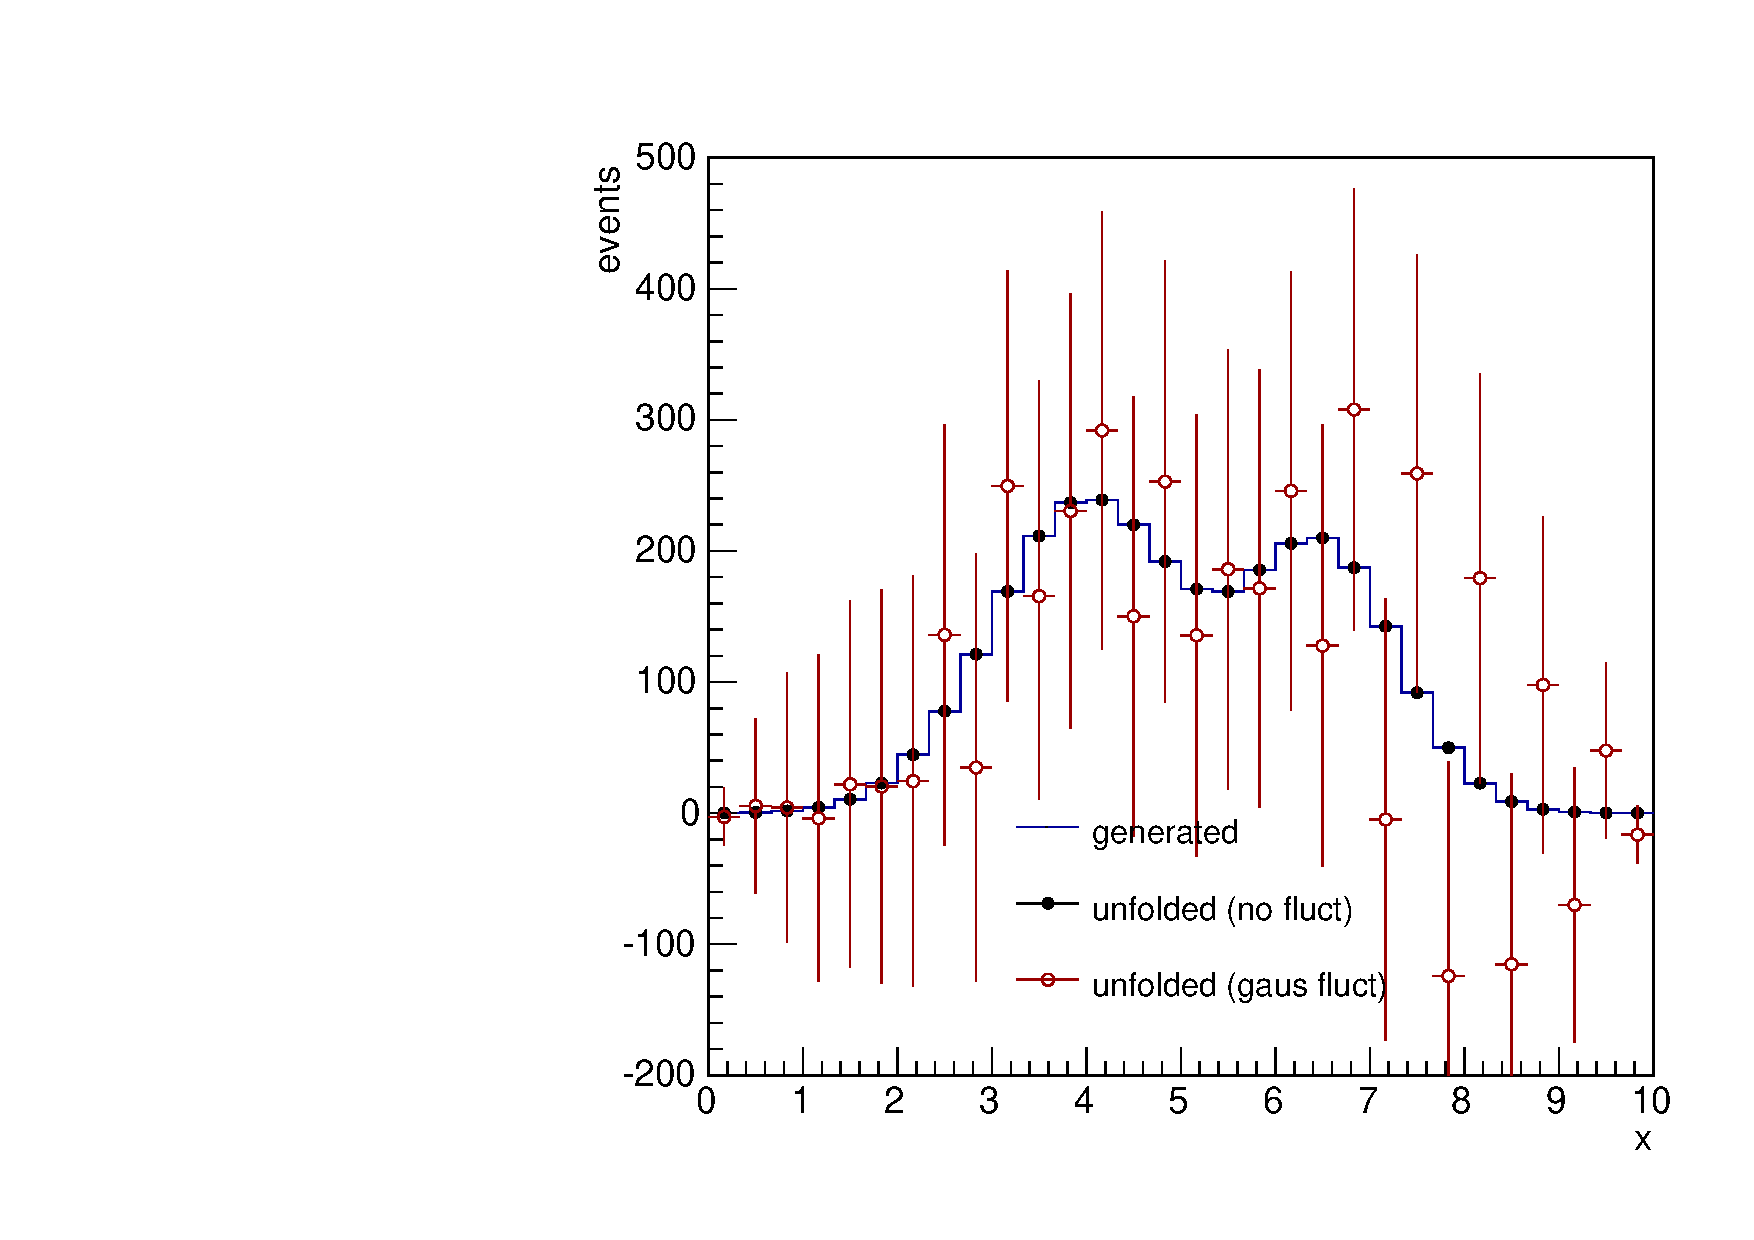
\includegraphics[width=0.618\textwidth]{figs/gen-unfold.pdf}
	\caption{ \label{fig:sol1} The two unfolded distribution compared with the one used to generate them.}
\end{figure}

\FloatBarrier
\end{document}
